\documentclass[12pt]{article}
 
\usepackage[margin=1in]{geometry} 
\usepackage{amsmath,amsthm,amssymb}
\usepackage{hyperref}
\usepackage{graphicx}
\usepackage{xcolor}
\usepackage[many]{tcolorbox}
\tcbuselibrary{listings}
\usepackage{listings}

\definecolor{lg}{HTML}{f0f0f0}

\newtcblisting{pycode}{
    colback=lg,
    boxrule=0pt,
    arc=0pt,
    outer arc=0pt,
    top=0pt,
    bottom=0pt,
    colframe=white,
    listing only,
    left=15.5pt,
    enhanced,
    listing options={
        basicstyle=\small\ttfamily,
        keywordstyle=\color{blue},
        language=Python,
        showstringspaces=false,
        tabsize=2,
        numbers=left,
        breaklines=true
    },
    overlay={
        \fill[gray!30]
        ([xshift=-3pt]frame.south west)
        rectangle
        ([xshift=11.5pt]frame.north west);
    }
}

\lstset{
    language=Python,
    basicstyle=\small\ttfamily,
}

 
\begin{document}
 
\title{Exercise 1}
\author{Jari Mattila - 35260T\\
ELEC-E8125 - Reinforcement Learning}

\maketitle
\section*{Task 1 - 5 points}

To cite works, put them in the template.bib file and use~\cite{sutton2018reinforcement}.
\newline

\noindent  
The result is as expected if all test episodes are successful in keeping the balance for 200 timesteps   


\begin{figure}[h] 
	\centering  % Remember to centre the figure
    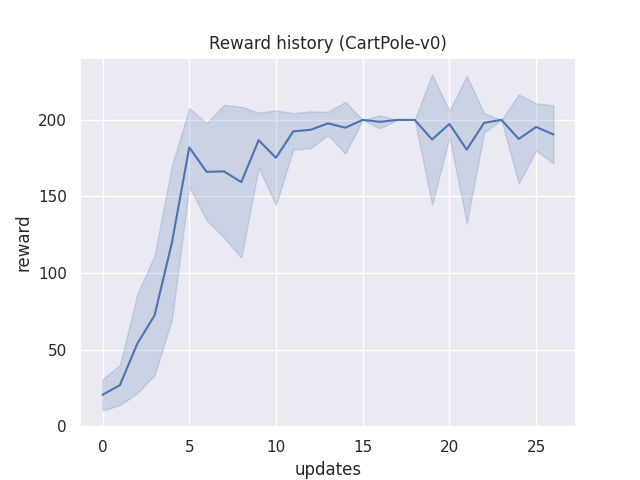
\includegraphics[width=0.9\columnwidth]{img/Figure_task1.png}
	\caption{Cartpole training with 200 episodes.}
	\label{fig:fig1}
\end{figure}


\section*{Question 1.1 - 15 points}

Can the same model, trained to balance for 200 timesteps, also balance the pole for 500 timesteps? Briefly justify your answer.
\newline

\noindent
Running the balancing test with a different number of episodes gives the following result:  
\newline
\indent
\# of episodes 200: Average test reward: 200.0 episode length: 200.0
\newline
\indent
\# of episodes 500: Average test reward: 494.644 episode length: 494.644
\newline
\indent
\# of episodes 1000: Average test reward: 832.828 episode length: 832.828
\newline

\noindent
The result is as expected if all test episodes are successful in keeping the balance for 200 timesteps.
\newline
\newline
\noindent
Yes, the same model trained to balance for 200 timesteps can also be used to balance the pole for 500 timesteps. 
You can clearly see from Figure \ref*{fig:fig1} that 500 as the number of episodes (i.e. train--episodes) for training (shown as the number of updates in the figure) is more than enough to learn the behaviour. 

\section*{Task 2 - 10 points}

The average test rewards over three trial/episodes are as follows:
\newline

Average test reward: 497.818 episode length: 497.818
\newline
\indent
Average test reward: 489.306 episode length: 489.306
\newline
\indent
Average test reward: 497.082 episode length: 497.082

\section*{Question 1.2 - 15 points}

Are the behavior and performance of the trained model the same every time?
Why/why not? Analyze the causes briefly.
\newline

\noindent
The behaviour and performance of the trained models are not exactly the same every time because the training procedures are stochastic random processes. However, the overall difference between the average test results is rather small because the averaging is over 500 independent trials/episodes.


%\pagebreak
\section*{Question 2 - 10 points}

Figure 2 shows the mean and standard deviation throughout 100 independent training procedures. You can notice that there is a large variance between the runs of the script.
\newline

Why is this the case? What are the implications of this stochasticity, when it comes to comparing reinforcement learning algorithms to each other? Please explain.
\newline

\noindent
As shown in Figure 2, the performance difference between the individual training procedures is rather large that is due to the stochasticity of the training processes. This is indicated by a large standard deviation (variance) between the individual processes. Comparing different RL algorithms to each other is possible using the average results (expected values). If the average results are computed over sufficiently many independent trials/episodes then the comparison of different algorithms should be valid. In Figure 2, the average of the reward curves is shown as a dark emphasized curve that would be easily comparable to other variations of the algorithm.  



\pagebreak
\section*{Task 3 - 20 points}

\subsection*{1. Reach the goal point located in x=[1.0,1.0]}
The embed code snippets in the report, you can use the \texttt{pycode} environment.

\begin{pycode}
def get_reward(self, prev_state, action, next_state):
        # Cartesian position of the end-effector
        cartesian_pos = self.get_cartesian_pos(next_state)
  
        # Distance between the position of the end-effector and the goal point [1.0,1.0]
        terminal_distance = np.sqrt(np.sum((cartesian_pos - self.goal)**2))

        is_terminal = terminal_distance < self.termination_threshold

        # Reward is 0 if the goal is achieved - otherwise -1
        reward = -1
        if is_terminal: 
            reward = 0

        return reward
\end{pycode}

\noindent  
The plot of this reward function is as follows: 

\begin{figure}[h] 
	\centering  % Remember to centre the figure
    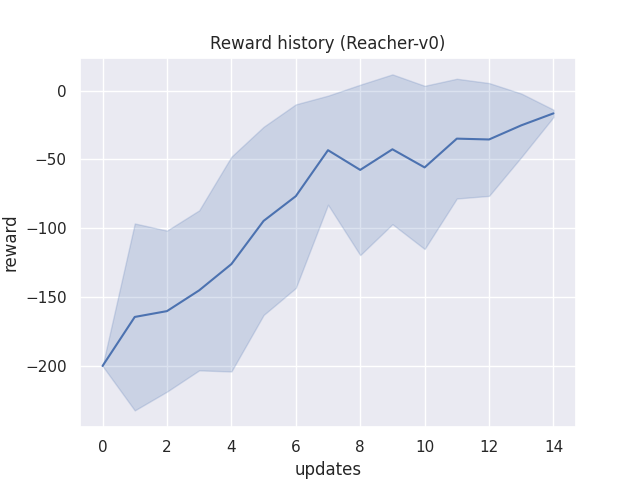
\includegraphics[width=0.8\columnwidth]{img/Figure_task3_1.png}
	\caption{Reacher training with 200 timesteps per episode.}
	\label{fig:fig31}
\end{figure}


\pagebreak
\section*{Task 4 - 10 points}

Now, let us visualize the reward function for the first behavior (reaching the goal [1,1]). Plot the values of the first reward function from Task 3 and the learned best action as a function of the state (the joint positions). 

%You can use the plot_rew.py script as a starting point.
%Make sure you include the plots in your report!

\begin{figure}[h] 
	\centering  % Remember to centre the figure
    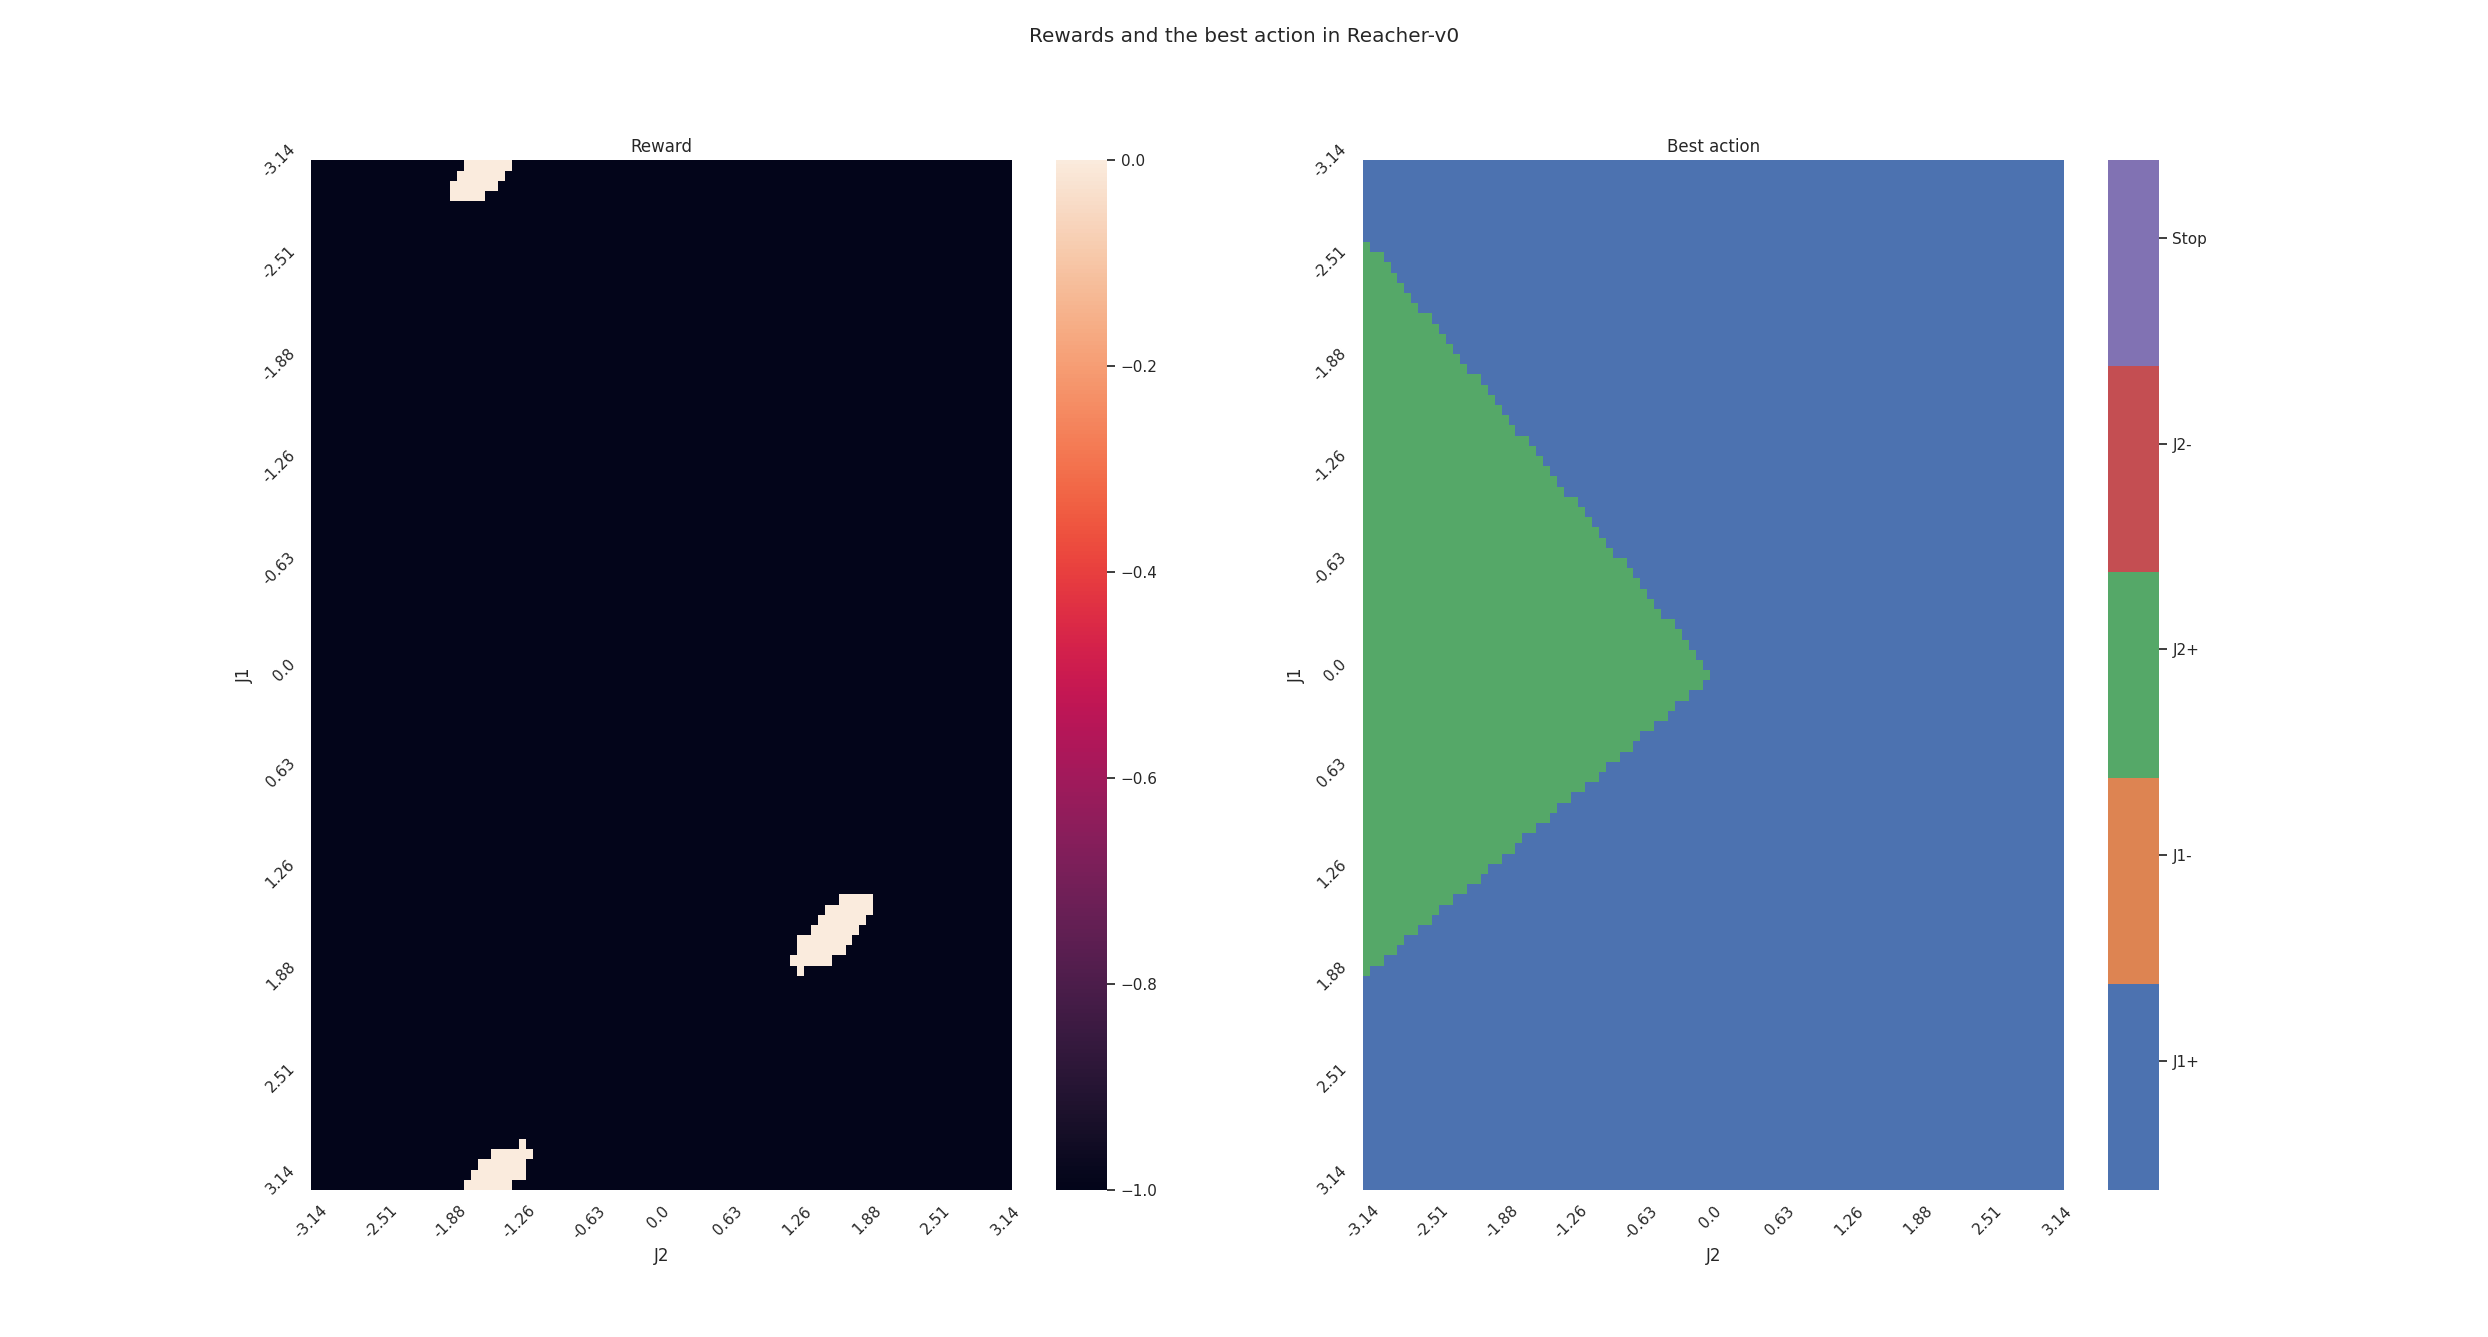
\includegraphics[width=0.9\columnwidth]{img/Figure_task4.png}
	\caption{The learned best action as a function of the state (the joint positions).}
	\label{fig:fig4}
\end{figure}


\section*{Question 3}

Analyze the plots in Task 4.


\section*{Question 3.1 - 5 points}

Where are the highest and lowest reward achieved?
\newline

\noindent
The highest rewards (=0.0) is achieved in in the lightest areas/spots of Figure \ref*{fig:fig4} (see the Reward plot on the left). As an example, one such point is $j_1 \approx 3.14$ and $j_2 \approx [-1.88,-1.26]$. The lowest reward (=-1.0) in Figure \ref*{fig:fig4} are achieved in the black area.



\section*{Question 3.2 - 10 points}

Did the policy learn to reach the goal from every possible state (manipulator
configuration)? Why/why not?
\newline

\noindent
No, the policy didn't learn to reach the goal from every possible state (manipulator configuration). It is obvious that only some manipulator configurations are possible for reaching the goal point [1,1], see e.g. the light spots of Figure \ref*{fig:fig4} (the Reward plot on the left).


\pagebreak


\bibliographystyle{ieeetr}
\bibliography{template}  % Modify template with your bibliography name
\end{document}
